\ylDisplay{Silindrilised anumad} % Ülesande nimi
{Jaan Kalda} % Autor
{lõppvoor} % Voor
{2014} % Aasta
{G 8} % Ülesande nr.
{9} % Raskustase
{
% Teema: Dünaamika
\ifStatement
\begin{wrapfigure}{r}{0.07\textwidth}%
\vspace{-15pt}
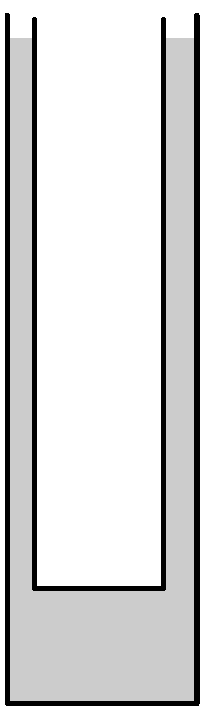
\includegraphics[width=1\linewidth]{2014-v3g-08-cylinders}
\end{wrapfigure}

Silindriline anum siseraadiusega $R = \SI{30}{mm}$ on täidetud veega. Teine tühi silindriline anum raadiusega $r =\SI{25}{mm}$, mille mass on tühiselt väike, on surutud koaksiaalselt suurema silindri sisse nii, et selle vettesukeldunud osa pikkus $L = \SI{300}{mm}$ (vt joonist). Leidke sisemise silindri kiirendus vahetult pärast seda, kui see vabaks lastakse. Vee pindpinevuse ning viskoossusega arvestada pole tarvis.
\fi


\ifHint
Üks võimalus sisemise silindri kiirenduse leidmiseks on rakendada virtuaalse nihke meetodit. Selle jaoks tuleb vaadelda, kuidas muutub süsteemi kineetiline ja potentsiaalne energia siis, kui sisemine silinder kerkib vahemaa $x$ võrra. Olles avaldanud süsteemi koguenergia $x$ kaudu, võib sellest tuletise võtta ning võrdsustada selle \num{0}-ga.
\fi


\ifSolution
Kui tühi anum kerkib vahemaa $x$ võrra, siis tema all vabaneb ruumala
$\pi r^2 x$, mille täidab silindritevahelisest ruumist
pärit vesi.  Vajugu nivoo vahemaa $y$ võrra; ruumalade võrdsuse tõttu
$\pi r^2 x = \pi (R^2-r^2) y$, seega
$$y=x\frac {r^2}{R^2-r^2}.$$
Kui $x\ll L$, siis süsteemi potentsiaalne energia väheneb vee ülevalt
alla ümberpaigutumise tõttu suuruse
$$E_p=g\rho \pi r^2 x L$$
võrra.
Energia balansis võime ignoreerida sisemise silindri otsa juures
toimuva vee liikumise kineetilist energiat, kuna selles osaleva vee hulk on väga väike võrreldes langeva vee hulgaga.
Seetõttu vee kineetiline energia
$$E_k=\frac 12 \rho \pi (R^2-r^2) L\dot y^2,$$
kus $\dot y$ tähistab $y$ tuletist aja järgi.
Võttes energia jäävuse seadusest  $gr^2x=\frac 12(R^2-r^2)\dot y^2$
tuletise aja järgi, leiame
$$gr^2\dot x=(R^2-r^2)\dot y\ddot y.$$
$x$ ja $y$ vahelise seose tõttu kehtib võrdus $r^2\dot x=(R^2-r^2)\dot
y$, mistõttu
$$\ddot y = g\Rightarrow \ddot x = g\frac
{R^2-r^2}{r^2}\approx\SI{4,3}{m/s^2}.$$
\fi


\ifEngStatement
% Problem name: Cylindrical vessels
\begin{wrapfigure}{r}{0.06\textwidth}%
\vspace{-15pt}
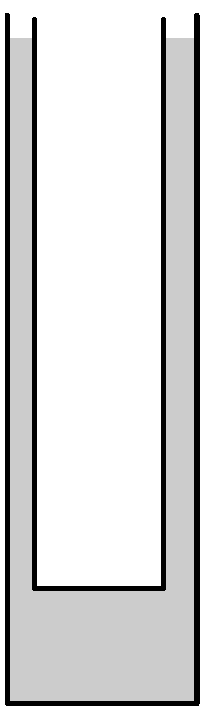
\includegraphics[width=0.06\textwidth]{2014-v3g-08-cylinders}
\end{wrapfigure}
A cylindrical vessel of inside radius $R = \SI{30}{mm}$ is filled with water. Another empty cylindrical vessel of radius $r =\SI{25}{mm}$ and with an insignificantly small mass is coaxially pressed into the bigger cylinder so that the length of the part in the water is $L = \SI{300}{mm}$ (see figure). Find the acceleration of the inner cylinder right after when it is let free. You do not have to account for the water’s surface tension or viscosity.
\fi


\ifEngHint
One way to find the acceleration of the inner cylinder is to apply the method of virtual displacement. For this you should observe how the kinetic and potential energy of the system changes when the inner cylinder rises by a distance $x$. After expressing the total energy of the system by $x$ you can find its derivative and equalize it with 0.
\fi


\ifEngSolution
If the empty vessel rises by a distance $x$ then a volume $\pi r^2 x$ is released under it, this is filled by the water from the space between the cylinders. Let the level sink by a distance $y$; due to the volumes being equal $\pi r^2 x = \pi (R^2-r^2) y$, therefore
$$y=x\frac {r^2}{R^2-r^2}.$$
If $x\ll L$ then due to the water’s placement from up to down the potential energy of the system decreases by
$$E_p=g\rho \pi r^2 x L$$ 
In the energy balance we can ignore the kinetic energy of the water movement happening at the end of the inner cylinder because the water amount there is very small compared to the amount of water sinking. Thus, the kinetic energy of the water
$$E_k=\frac 12 \rho \pi (R^2-r^2) L\dot y^2,$$ 
Where $\dot y$ marks the time derivative of $y$. Taking a derivative of time from the conservation energy $gr^2x=\frac 12(R^2-r^2)\dot y^2$, we find
$$gr^2\dot x=(R^2-r^2)\dot y\ddot y.$$ 
Due to the relation between $x$ and $y$ the equality $r^2\dot x=(R^2-r^2)\dot
y$ applies, therefore
$$\ddot y = g\Rightarrow \ddot x = g\frac
{R^2-r^2}{r^2}\approx\SI{4,3}{m/s^2}.$$
\fi
}